\chapter{Semantics-First Approach to Clinical Decision Support}

In \autoref{chapter:introduction}, we explained that, despite
advances in medicine, mortality and costs associated with preventable
medical errors (\PMEs{}) remain unacceptably high. In
\autoref{chapter:background}, we explained how systems that
assist healthcare practitioners (\HCPs{}) with situation-specific
advice based on evidence-based best practice guidelines (\BPGs{}),
called clinical decision (\CDSSs{}) can reduce both mortality
and costs associated with \PMEs{}. But, despite their potential,
the uptake of such systems in practice is hindered by challenges
that were introduced in \autoref{sec:hurdles-cdss-adoption}, and
discussed in depth in \autoref{chapter:hurdles-cdss-adoption}.
In brief, the following challenges (Cs) were outlined:
\begin{enumerate}[label=C\arabic*.]
\itemsep0.0em
\item Absence of systematic ways of \emph{validating content}
in a \emph{reliable}, \emph{accessible} and \emph{updateable} manner.
\item Lack of \emph{reliable}, \emph{shareable} \CDSS{} content
that can be easily adopted across healthcare organizations and their (Information
Technology) \IT{} systems.
\item Technical difficulties of sharing due to \emph{need for
  adaptation} to diverse Electronic Health Records (\EHR) systems.
\item \emph{Suboptimal} User Interfaces (\UIs), implementation choices and
workflows.
\end{enumerate}

\begin{figure}[th!]
  \centering
  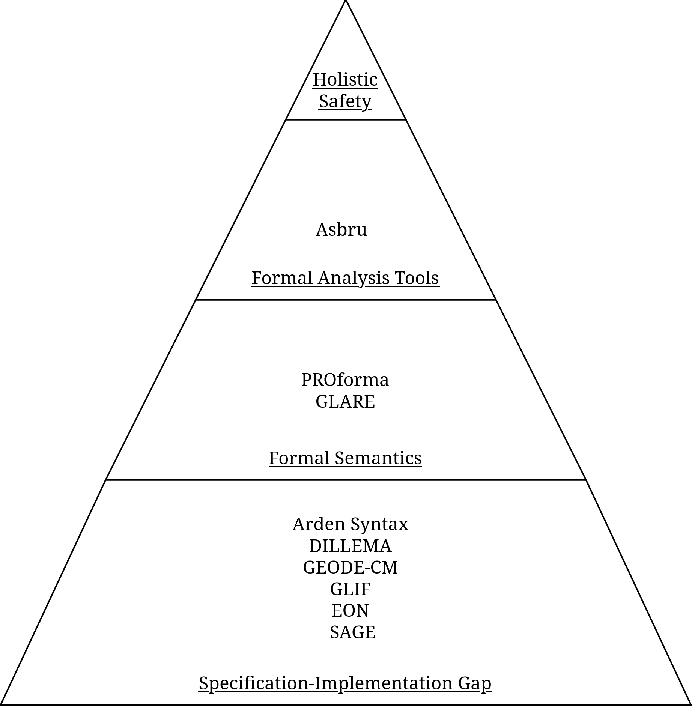
\includegraphics[width=0.5\textwidth]{pyramid}
  \caption{Existing \DSLs{} for Computer Interpretable Guidelines}\label{fig:existing-work-pyramid}
\end{figure}

Over the years, significant progress has been made towards
addressing these challenges. In \autoref{chapter:related-work},
we discussed how existing approaches have attempted to
address said challenges, and their limitations. Specifically,
in \autoref{sec:related-work-discussion}, we outlined major
themes that these approaches adopt to tackle these challenges.
This is further illustrated by the pyramid diagram in \autoref{fig:existing-work-pyramid}, where aforementioned themes are
underlined in the pyramid's various rungs.
As is typical, approaches that appear in higher rungs also
have characteristics of ones below them. For example, while guidelines expressed in
the Arden Syntax eliminate the specification-implementation gap by being
both \HCP{}-comprehensible and interpretable, they cannot be formally analyzed
due to lack of analysis tools in the ecosystem. Asbru-based guidelines
on the other hand not only eliminate the specification-implementation gap, but can also be
formally analyzed using support for KIV-based verification in the Asbru
ecosystem (see \autoref{sec:kiv-verification}).

As is evident in \autoref{fig:existing-work-pyramid}, no
existing approach covers the \say{holistic safety} rung of the pyramid.
Recall from \autoref{sec:related-work-discussion} that we say an
approach tackles \say{holistic safety} if,
besides support for analyzing guidelines,
analysis and execution tools also have correctness guarantees.
In this work, we argue that such guarantees are necessary for
trustworthy \CDSSs{}. We attempt to address \say{holistic safety}
systematically by developing a \emph{semantics-first approach} for
building clinical decision support systems. In this context, by semantics-first
we mean that:
\begin{itemize}
  \item The semantics of the programming language for defining said knowledge is
    formally defined, from which execution and analysis tools are derived in a
    correct by construction manner, leading to holistic safety.
  \item The semantics of medical knowledge are expressed accurately.
\end{itemize}
At the core of our approach is a novel domain-specific language for expressing
medical knowledge called $\MediK{}$ (pronounced Medi-Kay). By being comprehensible to domain experts
in medicine, $\MediK{}$-based computer interpretable guidelines can serve
both as a guideline's non-executable \HCP{}-comprehensible description, i.e.,
the specification, and its encoding in a computable medium, i.e., the
implementation, thereby eliminating any specification-implementation gap.

The remainder of this chapter is structured as follows:
\autoref{sec:semantics-first} briefly describes the semantics-first philosophy.
Next, \autoref{sec:k-framework} describes $\K$ -- the language semantic
framework that $\MediK{}$'s are expressed in. Finally,
\autoref{sec:semantics-first-pitfalls} describes potential pitfalls
of following the semantics-first philosophy.

\section{Semantics-First Approach}\label{sec:semantics-first}

The semantics-first approach prescribes a systematic way of
developing programming languages. Instead of implementing
tools for a language, such as interpreters, compilers and
model checkers in ad-hoc manner, the approach states that the
first step in developing said tools must be to formally define
the language's semantics. As show in \autoref{fig:semantics-first},
once defined, all tools for the language
can then be automatically derived from the semantics. Moreover, since
the tools utilize the semantics, they are, by definition,
correct-by-construction.

While following the semantics-first philosophy might seem like an obvious choice
in language design, its adoption in practice is far from ideal.
Conventional practice in the programming language and formal
methods community is still to develop analysis and execution tools for each
programming language from scratch \cite{ChenSETSS19}, as illustrated
in \autoref{fig:conventional-pl-development} from
\cite{ChenSETSS19}. But, this approach has several
disadvantages:
\begin{itemize}
  \item Implementing tools that perform the same function for
    different languages incurs unnecessary development and maintenance cost.
    As shown in \autoref{fig:conventional-pl-development}, if there are
    $l$ languages, where each has $t$ tools, then a total of $l \times t$
    tools have to be developed and maintained over time.
  \item Tools are often based on informal descriptions of language semantics,
    leaving developers to extrapolate finer details of the language's semantics,
    leading to inconsistencies.
    For instance, in \cite{ParkPLDI15}, it was found
    that ECMAScript 5.1-compliant JavaScript engines
    in mainstream web browsers behaved differently from each other
    for certain complex JavaScript programs.
  \item As newer versions of a language are introduced, each
    tool for the language has to be updated to ensure support for the latest
    version. This again results in duplicated work.
\end{itemize}
\begin{figure}[t!]
  \centering
  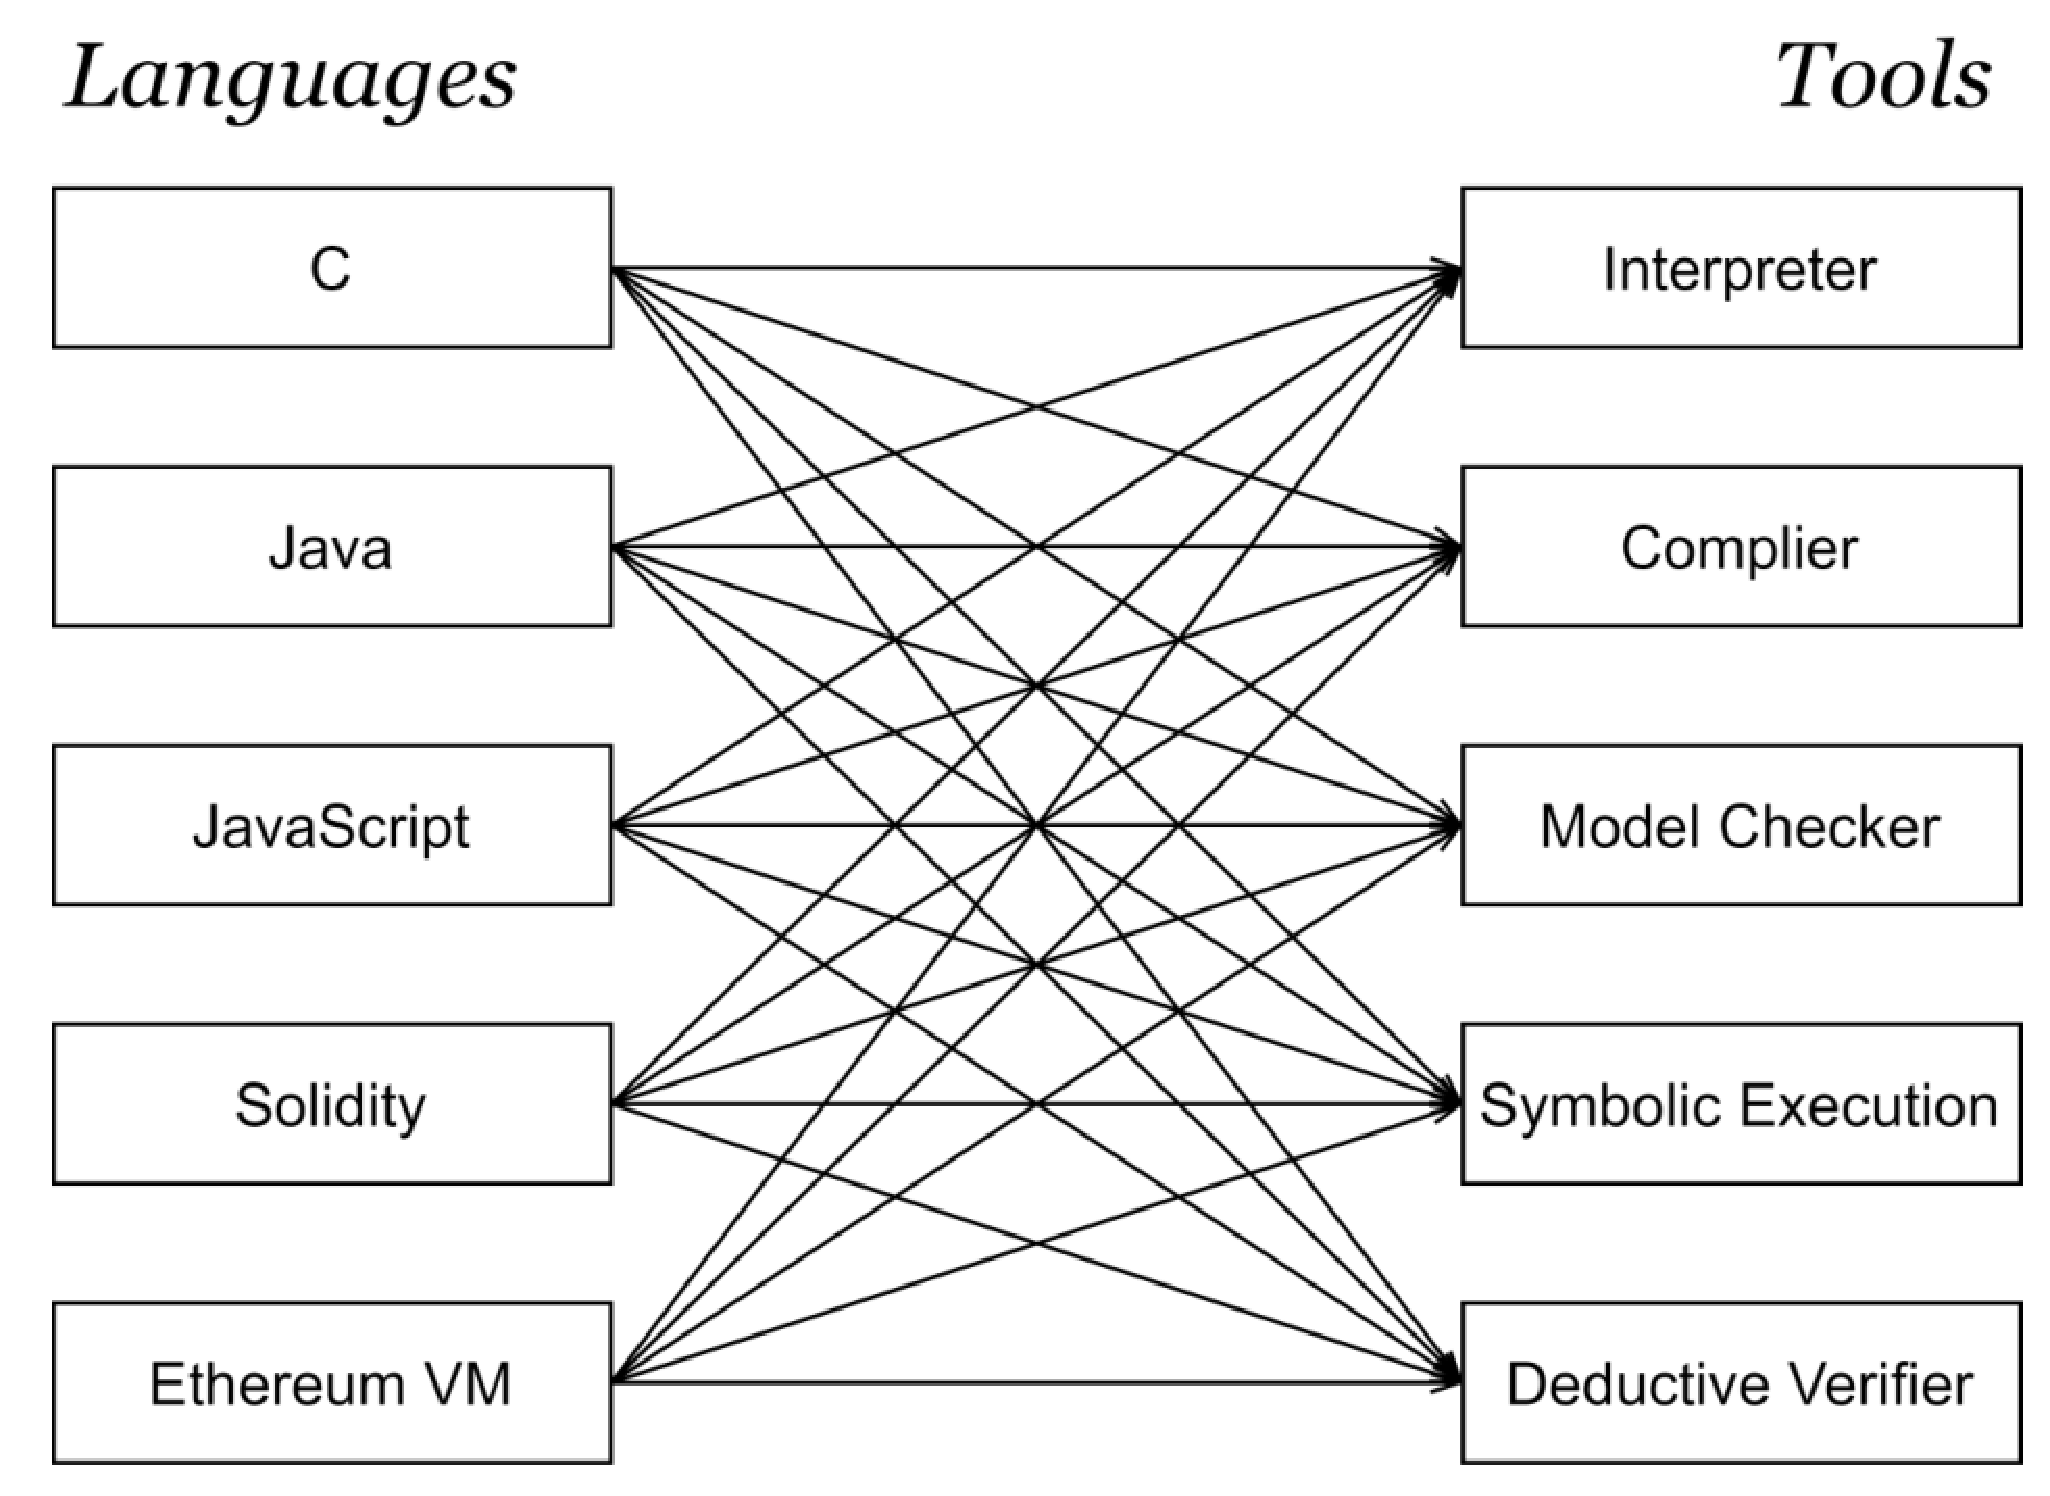
\includegraphics[width=0.6\textwidth]{conventional-pl-development}
  \caption{State-of-Art in Programming Language Design}\label{fig:conventional-pl-development}
\end{figure}

\subsection{Why build \CDSSs{} using Semantics-First?}

In section \ref{sec:semantics-first}, we described benefits
of using the semantics-first approach for developing regular programming
language. But, these differences become starker when semantics-first
is compared against the conventional approach shown in \autoref{fig:conventional-pl-development} in context of domain-specific language for
expressing medical guidelines. Specifically, as such a language will be utilized
in safety-critical settings, it is vital that the language:
\begin{itemize}
  \item Has an \emph{unambiguous}, \emph{formal}
    semantics that can serve as a reference for developing tool support for it.
    This is necessary to ensure that
    tools are free of behavioral inconsistencies due to ambiguities in the
    semantics.
  \item Is supported by a rich formal analysis tools that can
    be used to analyze programs.
    Implementing such tools from scratch would require significant effort.
  \item Can evolve quick to incorporate
    \begin{enumerate*}[label=(\roman*)]
      \item lessons from expressing medical guidelines in it, and,
      \item \HCP{} feedback, specifically regarding comprehensibility.
    \end{enumerate*}
    This can be challenging when using the approach shown in \autoref{fig:conventional-pl-development}, as
    every change to the language's semantics would require corresponding
    changes to all relevant tools, and additional effort to maintain
    different versions, making the development process extremely tedious.
\end{itemize}

\section{The $\K{}$ Framework}\label{sec:k-framework}

In this section, we introduce $\K{}$: a rewrite-based executable semantics
in which programming languages can be defined through configurations and rules
\cite{KframeworkUrl}. Once the semantics of a programming language has been
defined, $\K{}$ automatically generates all tools depicted in \autoref{fig:semantics-first}, such as an interpreter, compiler,
model-checker and deductive verifier for the language. $\K{}$ has been successfully
utilized to formalize semantics of large real-world languages, such as
C \cite{HathhornPLDI15}, Java \cite{BogdanasPOPL15} and
Javascript \cite{ParkPLDI15}, and analyze non-trivial programs
\cite{StefanescuOOPSLA16,ParkFSE18}.

The remainder of this section introduces relevant features of
$\K{}$ by describing the $\K{}$ semantics of an example language called
Imp. This introduction to $\K{}$ provides necessary background
for upcoming chapters that discuss the $\MediK{}$ \DSL{} through the
use of $\K{}$ notation and concepts.

\subsection{Defining Languages in $\K$}\label{sec:semantics-in-k}

A typical $\K$ definition of a language consists of the following components:
\begin{itemize}
  \item Syntax: Defined in \BNF{}-like notation, and utilized by $\K$
    to generate a parser for the language.
  \item Configuration: Organizes the program execution state
    into units called \emph{cells} that may be nested.
  \item Rules: Operate over configuration segments and define program
    evolution via rewrites.
\end{itemize}
We now discuss aforementioned components in the context of the Imp
language. Imp is a simple imperative programming language
inspired by C and Java that supports arithmetic and boolean expressions and
statements such as variable declaration and assignment, branching (\inlineimp{if})
and looping (\inlineimp{while}).

\autoref{lst:imp-syntax} and \autoref{lst:imp-semantics},
define syntax and semantics of Imp respectively.
$\K{}$ code must be place inside an organizational unit called a
\inlinek{module} that has a name, and can import other \inlinek{module}(s).
For example, \inlinek{module IMP-SYNTAX ... endmodule}
between \autoref{lstline:imp-module-start} and
\autoref{lstline:imp-module-end} of \autoref{lst:imp-syntax} defines
a $\K{}$ \inlinek{module} named \inlinek{IMP-SYNTAX} containing Imp's
grammar. $\K{}$ provides builtin support for domains such as natural
numbers, integers, booleans and program identifiers
under a \inlinek{module} named \inlinek{DOMAINS}.
\autoref{lstline:imp-syntax-import} \inlinek{imports}
the syntax definition of $\K{}$'s \inlinek{DOMAINS} module
to enable parsing integers and booleans in Imp programs.

\begin{lstlisting}[float=ht,
  frame=single,
  style=ksty,
  language=k,
  numbers=left,
  numbersep=5pt,
  caption={Imp Syntax in $\K$},
  label={lst:imp-syntax}
]
module IMP-SYNTAX                                               @\label{lstline:imp-module-start}@
  imports DOMAINS-SYNTAX                                        @\label{lstline:imp-syntax-import}@
  syntax AExp  ::= Int | Id                                     @\label{lstline:imp-aexp-start}@
                 | "-" Int
                 | AExp "/" AExp              [left, strict]    @\label{lstline:imp-aexp-div}@
                 | "(" AExp ")"               [bracket]
                 > AExp "+" AExp              [left, strict]    @\label{lstline:imp-aexp-end}@
  syntax BExp  ::= Bool
                 | AExp "<=" AExp             [seqstrict]
                 | "!" BExp                   [strict]
                 | "(" BExp ")"               [bracket]
                 > BExp "&&" BExp             [left, strict(1)] @\label{lstline:imp-bexp-and}@
  syntax Block ::= "{" "}"
                 | "{" Stmt "}"
  syntax Stmt  ::= Block                                        @\label{lstline:imp-stmt-block}@
                 | Id "=" AExp ";"            [strict(2)]       @\label{lstline:imp-stmt-assgn}@
                 | "if" "(" BExp ")"
                   Block "else" Block         [strict(1)]
                 | "while" "(" BExp ")" Block                   @\label{lstline:imp-stmt-while}@
                 > Stmt Stmt                  [left]            @\label{lstline:imp-stmt-comp}@
  syntax Pgm ::= "int" Ids ";" Stmt                             @\label{lstline:imp-pgm}@
  syntax Ids ::= List{Id,","}                                   @\label{lstline:imp-ids}@
endmodule                                                       @\label{lstline:imp-module-end}@
\end{lstlisting}

\emph{Syntax} in $\K{}$ is defined using BNF-like notation; terminals are enclosed
in quotes, and non-terminals begin with an uppercase. For example,
consider the declaration of Imp arithmetic expressions between
\autoref{lstline:imp-aexp-start} and \autoref{lstline:imp-aexp-end}. On
\autoref{lstline:imp-aexp-start} $\K$'s builtin support
for integers (\inlinek{Int}) and program identifiers
(\inlinek{Id}) is used to support arithmetic expressions over program variables.
Beyond simply defining the syntax, $\K{}$ also allows assigning semantics to
constructs through the use of \emph{attributes} specified as a comma-separated list
inside square brackets (\inlinek{[..]}) placed immediately after the \BNF{} production.
For example, On \autoref{lstline:imp-aexp-div} and \autoref{lstline:imp-aexp-end},
the attribute \inlinek{left} is used to declare the
corresponding operator as left associative. The \inlinek{strict} attribute is used
to assign \emph{evaluation strategies}. Note its use
on \autoref{lstline:imp-aexp-div} and \autoref{lstline:imp-aexp-end}, signifying
that both operand sub-expressions must be completely evaluated before the
before the corresponding operator (\inlinek{/}, \inlinek{+}) is evaluated.
Note that the order in which the arguments are evaluated is non-deterministic,
and, all operands will be evaluated before the operator is evaluated.
To enforce a particular order, or, to choose a subset of the operands, a
list of operand positions specifying the desired order can be supplied to
\inlinek{strict}. For example, \inlinek{strict(2, 1)} would make $\K$
evaluate the second argument before the first. This is particularly
useful for defining constructs like short-curcuit \inlineimp{&&} boolean
expression on \autoref{lstline:imp-bexp-and}, where \inlinek{strict(1)}
ensures that the left operand is evaluated first, allowing the right to only
be evaluated if the left evaluates to \inlinek{true}.
Similarly, for an assignment statement on \autoref{lstline:imp-stmt-assgn}
the \inlinek{strict(2)} indicates that the second argument, i.e., the
expression to the right of the \inlineimp{=} sign must be evaluated before
the identifier on the left of the \inlineimp{=} is updated.

$\K{}$ also allows operator precedence to be specified as a part of the
syntax definition. On \autoref{lstline:imp-aexp-end},
the \inlinek{>} signifies that all preceding productions have higher precedence,
i.e., bind tighter, than the production for addition (\inlinek{+}).
Similarly, \autoref{lstline:imp-stmt-comp} defines statement composition.
Thus, preceding \inlinek{Stmt} productions
(\autoref{lstline:imp-stmt-block}-\autoref{lstline:imp-stmt-while}), that define
blocks (\inlinek{\{..\}}) and standalone statements such as variable assignment and
while loop have higher precedence, indicated by \inlinek{>} on \autoref{lstline:imp-stmt-comp}.

On \autoref{lstline:imp-pgm}, an Imp program is defined to start with a list of program variable
declarations (\inlinek{"int" Ids ";"}) followed by other statements. Note the
definition of a list of identifier (\inlinek{Ids}) on \autoref{lstline:imp-ids}. In $\K{}$,
\inlinek{List\{...\}} is used to define syntactic-lists, where the first
argument is the production of list elements, and the second the list de-limiter.
Thus, \inlinek{List\{Id, ","\}} defines a comma-separated list of program identifiers.

\begin{lstlisting}[float=hb,
  frame=single,
  style=ksty,
  language=k,
  numbers=left,
  numbersep=5pt,
  caption={$\K$ Semantics of Imp},
  label={lst:imp-semantics}
]
module IMP
  imports IMP-SYNTAX
  imports DOMAINS
  syntax KResult ::= Int | Bool

  configuration <T>
                  <k> $PGM:Pgm </k>
                  <state> .Map </state>
                </T>

// AExp
  rule <k> X:Id => I ...</k> <state>... X |-> I ...</state>
  rule I1 / I2 => I1 /Int I2  requires I2 =/=Int 0
  rule I1 + I2 => I1 +Int I2
  rule - I1 => 0 -Int I1
// BExp
  rule I1 <= I2 => I1 <=Int I2
  rule ! T => notBool T
  rule true && B => B
  rule false && _ => false
// Block
  rule {} => .   [structural]
  rule {S} => S  [structural]
// Stmt
  rule <k> X = I:Int; => . ...</k> <state>... X |-> (_ => I) ...</state>
  rule S1:Stmt S2:Stmt => S1 ~> S2  [structural]
  rule if (true)  S else _ => S
  rule if (false) _ else S => S
  rule while (B) S => if (B) {S while (B) S} else {}  [structural]
// Pgm
  rule <k> int (X,Xs => Xs);_ </k> <state> Rho:Map (.Map => X|->0) </state>
    requires notBool (X in keys(Rho))
  rule int .Ids; S => S  [structural]

endmodule
\end{lstlisting}


\section{Pitfalls of the Semantics-First Approach}\label{sec:semantics-first-pitfalls}
